% v0.2
\chapter{Bioinformatics methods}
\section{Sequence alignment}
In this section we would like to thoroughly explain what sequence alignment is, since it is one of the most essential tasks in bioinformatics.
We will describe two main types of sequence alignment, with emphasizing the differences.
We will also explain the basic algorithms used for solving these problems and we will also describe the heuristic method used in case the input is too big to be computable by standard approaches that guarantee optimal solution.
At the end of this section we will describe, how we used the algorithms in our analysis.

\subsection{Global alignment}
\subsubsection{Usage}
\emph{Global alignment} is commonly used for comparison between two sequences with roughly the same length.
This comparison can help us to discover mutations in a sequence that causes a certain phenotype \cite{}, or we can use the comparison to determine highly conserved regions with a potential to carry a gene \cite{}.
The relationships between conserved regions and mutations in certain sequences often serve as a basic assumption for construction of phylogenetic trees \cite{}.
Therefore, global alignment can tell us a lot about the nature of evolution.
Global alignment is also capable of calculating a similarity score for two sequences.

\subsubsection{Problem statement}
Let the input for the problem be a set of two sequences consisting of nucleotides, for example, $ X = ATTGATGG $ and $ Y = AATTCAAC $.
Then the output is represented as a matrix, where each row is one sequence with possible gaps between nucleotides.
We can see potential solutions in the Table (\ref{tab:potsol})

\begin{table}
  \centering
	\begin{tabular}{ l | r }
	\verb|A-TTGATGG| & \verb|-ATTG-ATGG| \\
	\verb|AATTCAAC-| & \verb|AATTCAAC--| \\
	\end{tabular}
  \caption{Global alignment examples}
  \label{tab:potsol}
\end{table}

As we can see, every alignment could have more than one valid solution.
Despite of multiple possible solutions, not every solution is of equal value to us.
We want to find the best possible solution to this problem and for this purpose, we implement a scoring scheme to determine what is the best solution.
\emph{Scoring scheme} consists of rules, which add numerical value to each column of pairwise alignment.
For example, we can evaluate match in column with score $+1$, mismatch with score $-1$ and alignment to gap with score $-1$.
With this scoring scheme, we can evaluate quality of a particular alignment.
For alignment on the left side of the Table (\ref{tab:potsol}), resulting score is $+1-1+1+1-1+1-1-1-1 = -1$ and for alignment on the right side of the Table (\ref{tab:potsol}) $-1+1+1+1-1-1+1-1-1-1 = -2$.
From this example we can see that according to our scoring scheme, alignment on the left is better.

\subsubsection{Scoring schemes}
In practice, we could use a more complex scoring scheme that better reflects reality.
For example, substitution between purines (adenine, guanine) or substitution between pyrimidines (cytosine, thymine) occur more often, because they do not require change in the number of rings in the chemical structure of these nucleotides \cite{}.
When we try to align two proteins, a more complex scoring scheme is inevitable.
Amino acids differ in many parameters such as: polarity, size and structure of their side chains.
This influences the probability of a substitution occurring between two amino acids.
Therefore, there is a higher probability that Leucine will be substituted for Isoleucine, rather than Aspartic Acid.
To solve the complexity of substitutions between amino acids, matrix BLOSUM62 (\ref{fig:blosum}) was created.
Another layer of complexity, that does a better job of reflecting reality is the \emph{affine gap penalty function}.
This reflects the fact that insertions and deletions do not usually occur only on one nucleotide, but often a longer region of DNA is deleted or inserted.
Affine gap penalty solves this issue by having a higher negative score for opening a new gap in alignment and a lower negative gap for extension of an already created gap \cite{}.

\begin{figure}[ht]
  \centering
	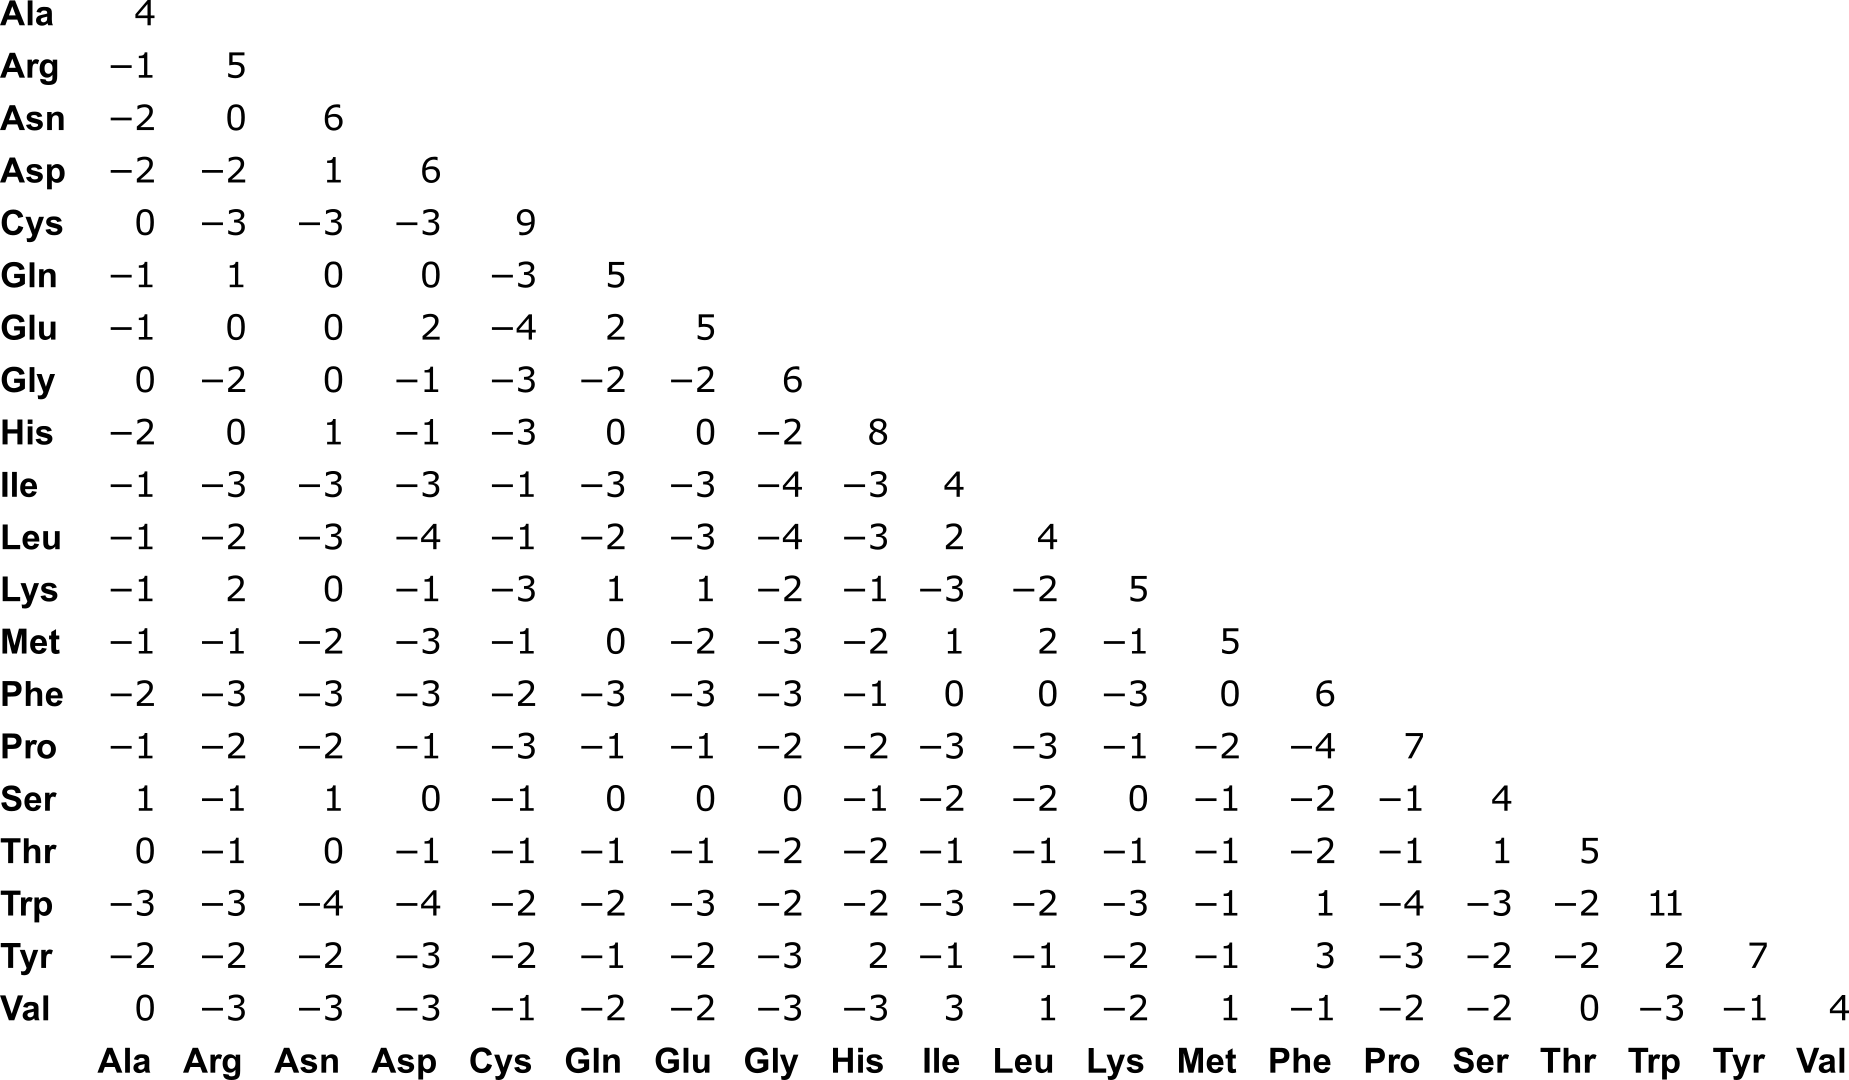
\includegraphics[width=\textwidth]{./images/blosum62.png}
  \caption{BLOSUM62}
  \label{fig:blosum}
\end{figure}

% end of session 16.04.2018

\subsubsection{Needleman-Wunsch algorithm}
For searching optimal global alignment, we usually use the Needleman-Wunsch algorithm.
It is an algorithm from a group of \emph{dynamic programming} algorithms.
This means that the main problem is divided into smaller problems, which are computable more easily and solutions to them are stored in memory.
At each occurrence of a small problem, we can look into stored solutions, where we can find it.
Then the main problem is reconstructed from already computed subproblems.
Dynamic programming algorithms offer saving time on computation at the expense of a higher memory usage.

\begin{figure}[ht]
  \centering
	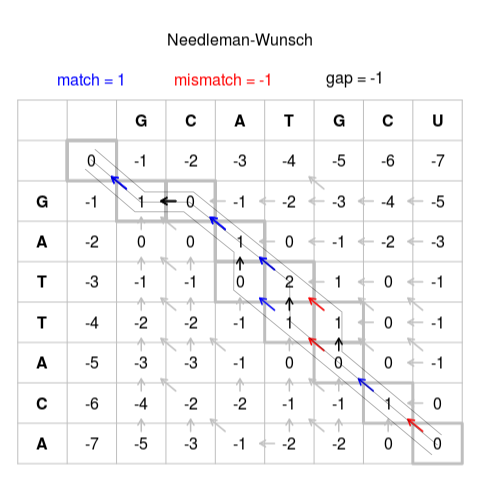
\includegraphics[width=\textwidth]{./images/needle_wunsch.png}
  \caption{Needleman-Wunsch}
  \label{fig:glal}
\end{figure}

Needleman-Wunsch algorithm produces a table as shown in the Figure (\ref{fig:glal}).
It starts by putting the first sequence we want to align to the first row and the second sequence to the first column.
Before each sequence there is one gap to cover the case if we would not want to align first letter of a particular sequence right from the beginning.
The table is then initialized with a series starting from 0 and decreasing by 1 each step on the second row and with the same series on the second column.
After initialization, the table starts to be filled from top left corner following this rule:\\
Into each cell $A_{i,j}$ write maximum of:
\begin{itemize}
\item $A_{i-1, j-1} + s()$,
\item $A_{i-1, j} + g()$,
\item $A_{i, j-1} + g()$,
\end{itemize}
where $s(X_i, Y_j)$ returns score of match/mismatch from scoring scheme and $g$ returns a score of the gap penalty (possibly affine gap).
The final score of the alignment can be found in the bottom right corner of the filled table.
Specific alignments can be found by tracking all possible paths to this value.
The time and space complexity of Needleman-Wunsch algorithm is $\mathcal{O}(nm)$, where $n$ is the length of the first sequence and $m$ is the length of the second sequence.

\subsection{Local alignment}
\subsubsection{Usage}
In comparison with global alignment, \emph{local alignment} search for regions inside sequences with high similarities and does not provide alignment from beginning to end.
It is generally useful when searching for a small subsequence inside a vast sequence.
For example, searching for a gene inside the whole bacterial genome.
It can be also used when comparing two different sequences and we want to find out if they contain any highly similar sequence.

\subsubsection{Problem statement}
Similarly to what we have done with the global alignment, in this problem we search for optimal local alignment according to the defined scoring system.
The difference is that we do not know where the alignment in both sequences starts and where it ends.
For example, $ X = TAATAACTCTCTGAATAA $ and $ Y = CGGCGGCGGTCTCTGCC $ can be aligned as in the Figure (\ref{tab:loal}) and the score is calculated just from the first aligned base to the last aligned base.

\begin{table}
  \centering
	\begin{tabular}{ c }
	\verb|--TAATAACTCTCTGAATAA| \\
	\verb%     	|||||| 	% \\
	\verb|CGGCGGCGGTCTCTGCC---| \\
	\end{tabular}
  \caption{Local alignment example}
  \label{tab:loal}
\end{table}

\subsubsection{Scoring}
Scoring of local alignment is similar to global alignment and we are allowed to use the same methods we use in the global alignment.
Since the score is calculated just from the first aligned base to the last aligned base, the score of our local alignment would be $+1+1+1+1+1+1 = 6$, because there are 6 matches ($+1$) and no gaps ($-1$) or mismatches ($-1$).

\subsubsection{Smith-Waterman algorithm}
Local alignment can be found with dynamic programming algorithm similar to Needleman-Wunsch algorithm.
This is called Smith-Waterman algorithm and there are only two changes compared to Needleman-Wunsch.
First change is that matrix is not initialized with decreasing series, but second row and second column are filled with zeroes.
Second difference is in the rule as follows:\\
Into each cell $A_{i,j}$ write maximum of:
\begin{itemize}
\item $0$,
\item $A_{i-1, j-1} + s()$,
\item $A_{i-1, j} + g()$,
\item $A_{i, j-1} + g()$.
\end{itemize}
After completing the table, we need to find the highest number in it.
This number is a resulting score of our local alignment.
Following the path similarly as in global alignment we can reconstruct the alignment.
The space and time complexity of this algorithm is also $\mathcal{O}(nm)$.

\subsection{Word methods}
Needleman-Wunsch and Smith-Waterman algorithms are sufficient for simple comparisons of sequences, but their time complexity is not good enough when we want to search through very long sequences that are common in genomics.
It is often the case that we want to find the most similar sequence to ours in enormous bioinformatics database containing genomes of large amount of organisms.
This is particularly useful if we want to find the potential source of our sequence or comparing it to all known proteins to get some indicators about its potential function.
For this purpose, various \emph{heuristic algorithms} were developed.
These algorithms do not guarantee finding the most optimal solution but are orders of magnitude faster and therefore usable also for searching in vast databases.

\subsubsection{BLAST}
%The basic algorithm consists of searching seeds from database on the query sequence and then extending those seeds into neighbouring bases.
%This approach provides orders of magnitude faster alignment method than classical Smith-Waterman algorithm \cite{smith_waterman} with comparable sensitivity.
\emph{Basic Local Alignment Search Tool} (BLAST) \cite{blast} is probably the most widely used tool in bioinformatics.
The algorithm distinguishes between target sequences and query sequences.
Target sequences are sequences from which we create a database of all included k-mers.
For every k-mer in every sequence we save its position.
For example, for sequence GATCGATAG and given $k=3$ we create database as follows:
\begin{verbatim}
GAT = 1, 5
ATC = 2
TCG = 3
CGA = 4
ATA = 6
TAG = 7
\end{verbatim}
Next, we find every k-mer from query sequence in the database.
The matching k-mers are called cores of alignment and serves as starting points for extending of alignment.
The extending is performed in a similar manner to that of Smith-Waterman algorithm.
The difference is that we do not need to search through the whole matrix, but we search for good alignments only in the immediate surrounding of cores.
Firstly, we extend cores without the possibility to insert any gaps into alignment.
Secondly, we can join these extended cores together using the gaps, if the resulting score will be bigger than before joining.

\subsubsection{E-value}
\emph{E-value} is used to assess the relevancy of the resulting alignment.
It can be interpreted as how many alignments in database could reach the same score or better purely by chance.
This means, the closer the E-value is to zero, the higher level of significance can be assumed.
E-value is automatically produced by BLAST.

\section{Data clustering}
In this section we will explain what is data clustering.
We will describe its use in data analysis and bioinformatics and how we used it in our program.
We will briefly define the problem and we will explain the algorithm used for solving it.
At the end, we will present three approaches used in our pipeline.

\subsection{Usage}
\emph{Data clustering} is used to group data according to similar characteristics.
In computational biology it can be used to cluster organisms to examine relationships between different groups or to study structure of population.
By clustering genes, we can investigate their functions and see which regions in sequence are responsible for them.
Clustering can also be used to distinguish different types of tissue or group drugs with similar effects according to their mechanism of action.

In our work, we clustered genes with sequential similarities.
We expected, that this approach will create clusters of genes with closely related functions.

\subsection{Definition of problem}
Clustering is a problem where we want to determine closely related entities and put them in distinct groups, also called clusters.
Cluster can be characterized by presence of many edges between cluster members.
Members from different clusters have lesser probability to be connected and the distance between them is usually longer.
Although, to intuitively understand clustering is not complicated, there exists a lot of clustering models with slightly different approaches, which makes exact general definition impossible.

\subsection{Markov Cluster Algorithm}
\emph{Markov Cluster Algorithm} \cite{} is searching for clusters by simulating random walks on the graph.
It assumes that these random walks will infrequently go from one cluster to different cluster and mostly will stay in the starting cluster.
The algorithm simulates random walks through the graph deterministically with two operations, expansion and inflation.
\emph{Expansion} corresponds with squaring of stochastic matrix, non-negative matrix where each column sums to 1 and entry $a_{ij}$ corresponds to probability of going from node $j$ to node $i$.
\emph{Inflation} is defined by entry-wise powering of stochastic matrix to the power of $r$, followed by scaling step to get stochastic matrix again.
It is observed that for $r>1$ inflation favors more probable walks over less probable walks.
Expansion can be interpreted as random walk with many steps.
Inflation then enlarges the effect of random walks within a cluster and reduces random walks across a different cluster.
By repeating expansion and inflation operations, the equilibrium is reached which produces the clusters.
These clusters do not contain any paths between each other and the only paths in graph are those within clusters.
This algorithm does not need any prior knowledge of clusters and resulting clusters emerge from the primary structure of the graph.
Furthermore, size of clusters can be regulated by changing parameter $r$ of inflation operation.
Bigger $r$ will cause algorithm to converge to equilibrium faster and will produce smaller resulting clusters.
In practice, $r$ from 1.2 to 5.0 is used.